\section[Conclusion]{\textbf{Conclusion}}

% % ============================================================
% % COMPUTATIONAL COST
% % ============================================================

% \begin{frame}{\small Computational Cost and Numerical Setup}
% \scriptsize

% \vspace{-0.15cm}

% \begin{columns}[T,onlytextwidth]

% % ============================================================
% % LEFT
% % ============================================================
% \begin{column}{0.61\textwidth}

% % ------------------------------------------------------------
% % COMPUTATIONAL COST
% % ------------------------------------------------------------
% \begin{block}{\scriptsize Computational Cost}
% \centering

% \renewcommand{\arraystretch}{1.25}
% \setlength{\tabcolsep}{3.5pt}

% \begin{tabular}{lccc}
% \toprule
% \textbf{Computation}
% & \textbf{Mesh Size}
% & \textbf{Wall Time}
% & \textbf{Hardware} \\
% \midrule

% NACA0012 -- Flow
% & $\sim45$M
% & 58 min
% & Trillium \\

% NACA0012 -- Droplets (7 bins)
% & $\sim45$M
% & 90 min
% & Trillium \\

% ONERA M6 -- Flow
% & $\sim25$M
% & 70 min
% & Trillium \\

% ONERA M6 -- Droplets (7 bins)
% & $\sim25$M
% & 53 min
% & Trillium \\

% \midrule

% Level Set
% & $\sim10$M
% & $\sim18$ min
% & Xeon w7-2595X (26 cores) \\

% \bottomrule
% \end{tabular}

% \end{block}

% \vspace{0.08cm}

% % ------------------------------------------------------------
% % REMARKS
% % ------------------------------------------------------------
% \begin{alertblock}{\scriptsize Remarks}
% \begin{itemize}
%     \item NACA0012 surface mesh is extracted from the L1 grid and
%     diagonalized, substantially increasing the number of surface elements.

%     \item ONERA M6 surface mesh is generated directly from CAD; flow
%     convergence required a small initial CFL followed by progressive ramping.

%     \item Significant room remains for optimization of the numerical setup
%     and meshing strategy (surface meshing, CFL, etc.).

%     \item A leading-edge element size of approximately $1$--$2\,\mathrm{mm}$
%     provides the best results for capturing complex ice features with the
%     level-set approach.
% \end{itemize}
% \end{alertblock}

% \end{column}

% \hfill

% % ============================================================
% % RIGHT -- SURFACE MESH
% % ============================================================
% \begin{column}{0.36\textwidth}

%     \centering

%     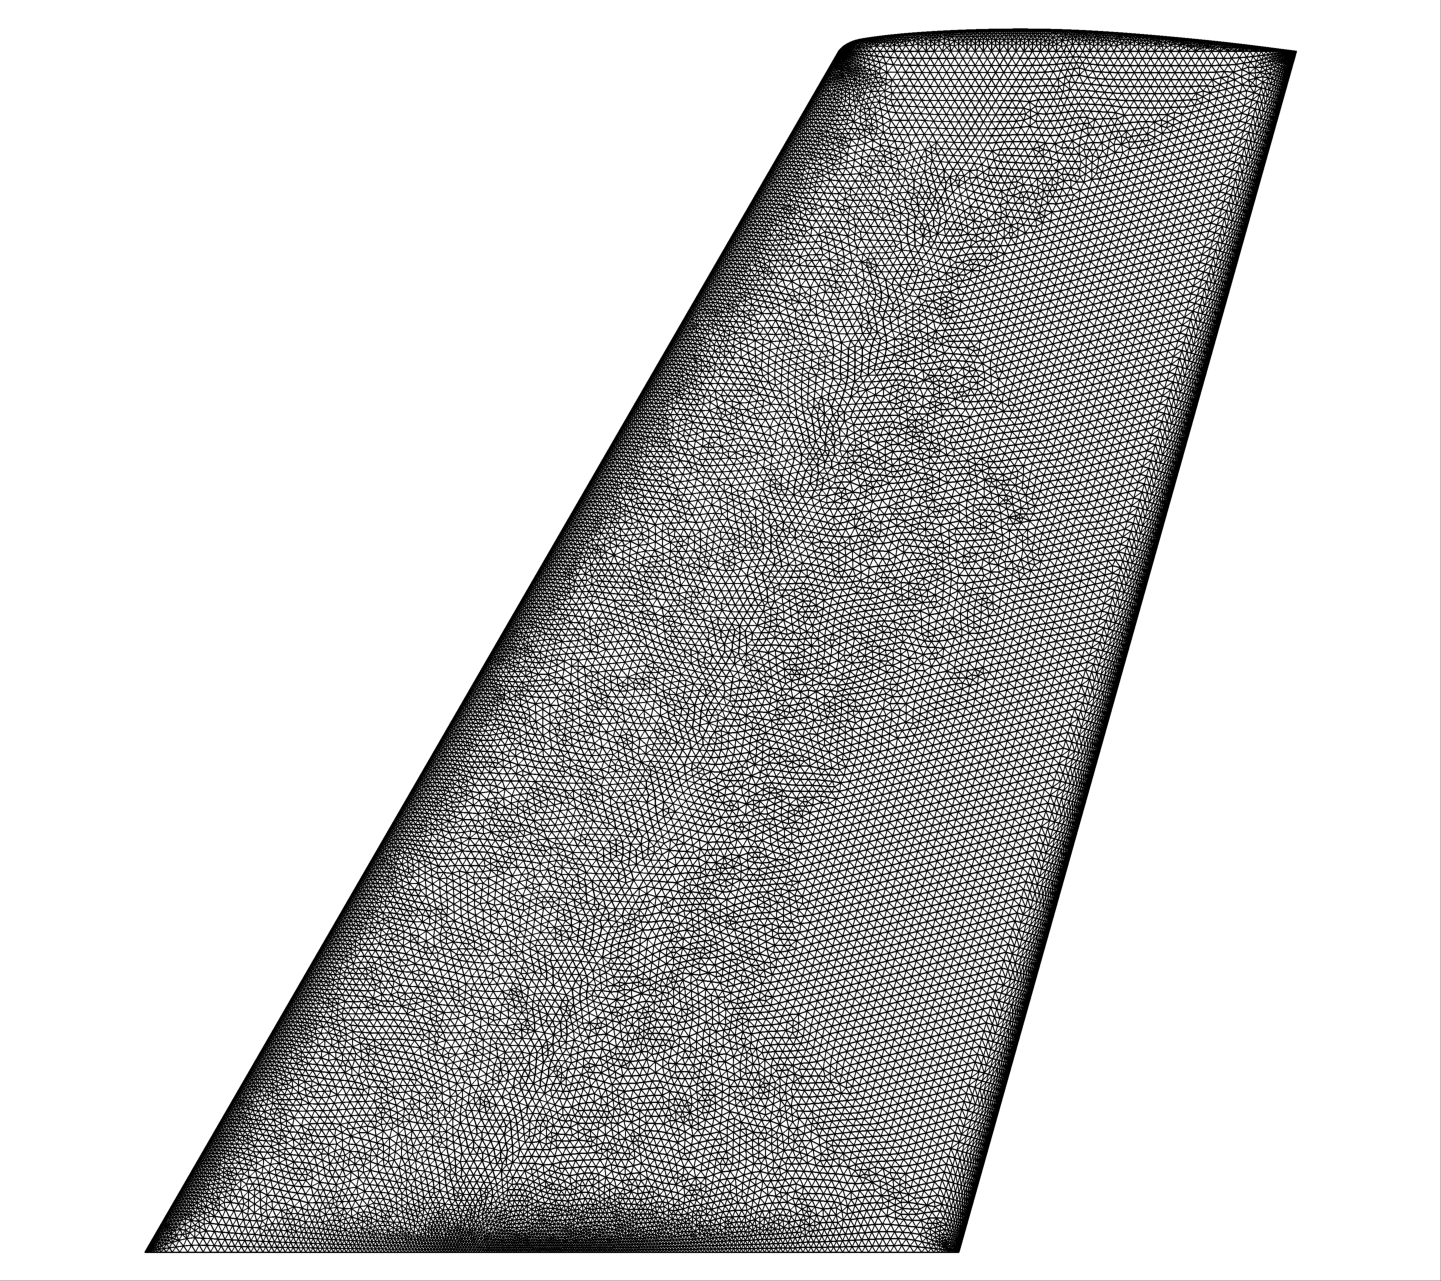
\includegraphics[
%         width=\textwidth,
%         height=0.76\textheight,
%         keepaspectratio
%     ]{FIGURES/ONERAM6/ICE_VIEWS/ONERA_M6_SURFACE_MESH.png}

%     \vspace{-0.05cm}

%     \textbf{ONERA M6 Surface Mesh}

%     \vspace{0.03cm}

%     {\scriptsize CAD-based triangular surface mesh}

% \end{column}

% \end{columns}

% \end{frame}

% ============================================================
% CONCLUSIONS
% ============================================================

\begin{frame}{\small Conclusions}
\scriptsize

% ------------------------------------------------------------
% GENERAL
% ------------------------------------------------------------
\begin{block}{\scriptsize General Findings}
\begin{itemize}
    \item Results are generally consistent across the grid hierarchy and well positioned within the IPW3 code-to-code envelope.
    \item Eulerian and Lagrangian droplet formulations show good agreement in collection efficiency and collected water mass.
\end{itemize}
\end{block}

\vspace{0.12cm}

% ------------------------------------------------------------
% NACA0012
% ------------------------------------------------------------
\begin{block}{\scriptsize NACA0012}
\begin{itemize}
    \item Single-layer ice shapes capture the experimental horn orientation well.
    \item Multilayer predictions show larger deviations in horn orientation, while capturing complex three-dimensional ice morphology.
\end{itemize}
\end{block}

\vspace{0.12cm}

% ------------------------------------------------------------
% ONERA M6
% ------------------------------------------------------------
\begin{block}{\scriptsize ONERA M6}
\begin{itemize}
    \item Single-layer ice shapes show limited grid sensitivity, with the largest deviations observed on L4.
    \item Multilayer simulations capture pronounced three-dimensional horn development and spanwise variations in the ice morphology.
\end{itemize}
\end{block}

\vspace{0.12cm}

% ------------------------------------------------------------
% OVERALL
% ------------------------------------------------------------
\begin{alertblock}{\scriptsize Overall}
\begin{itemize}
    \item CHAMPS provides a consistent end-to-end icing framework, with the level-set approach enabling complex three-dimensional ice geometries in multilayer simulations.
    \item Future work will focus on improving the roughness and ice-density models.
\end{itemize}
\end{alertblock}

\end{frame}

% ============================================================
% Acknowledgments
% ============================================================

\begin{frame}{\small Acknowledgments}
\scriptsize

\begin{itemize}
    \item This work is supported in part by a Bombardier/NSERC/CRIAQ Industrial Chair.

    \item Computations were performed on the Trillium supercomputer at the SciNet HPC Consortium, with computational resources provided through the Digital Research Alliance of Canada.

    %\item SciNet is funded by Innovation, Science and Economic Development Canada; the Digital Research Alliance of Canada; the Ontario Research Fund: Research Excellence; and the University of Toronto.
\end{itemize}

\end{frame}